\chapter{Work Package Tasks}
\label{ch:wptasks}

In this chapter, the high level tasks in each WP is discussed briefly. A reference architecture diagram is also given for each WP, this is meant to be seen as an early proposal and it is subjected to change.

\section{WP1: Service Descriptor Translator}

\subsection{Requirements definitions and architecture design}

The development of the SDT follows a microservice architecture. The architecture includes a message broker with a publish/subscribe model. The NSDs(yaml/JSON files) corresponding to the communicating MANO are published to the broker. The SDT subscribed to the broker, consumes the yaml/JSON files and translate one MANO NSD to the other schema and publish them back to the broker. These translated NSDs could be accessed by any other services through a REST API.
\begin{figure}[h]
	\centering
	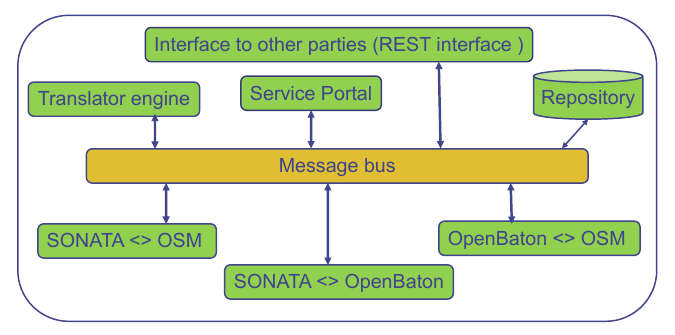
\includegraphics[width=0.9\linewidth]{figures/wp1Arch}
	\caption{Reference architecture for SDT \cite{WPDescriptionsPDF}}
	\label{fig:wp1arch}
\end{figure}

\subsection{Prototype implementation of SDT components}

After the concrete architecture is planned, a working prototype of the SDT including all the requisite components are modeled. This prototype is built as a standalone microservice.
\subsection{Proof of concept demonstration}

The functionality of the SDT will be demonstrated on virtual machines containing atleast two different MANO frameworks installed and deployed. 

\section{WP2: Service Descriptor Splitter}

\subsection{Requirements definition and architecture design}

  A publish/subscribe message broker model will be once again followed for the SDS implementation. The NSD(yaml/JSON file) is published to the message broker. A service graph splitter and a NSD splitter consumes the NSD from the broker and splits the NSD. The seperated NSDs are published back to the broker from where other services can consume those through REST API.
\begin{figure}[h]
	\centering
	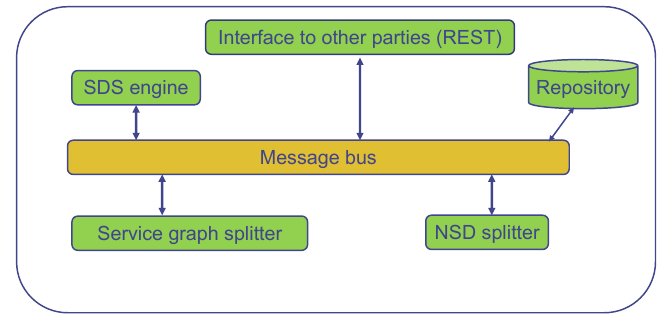
\includegraphics[width=0.9\linewidth]{figures/wp2Arch}
	\caption{Reference architecture for SDS \cite{WPDescriptionsPDF}}
	\label{fig:wp2arch}
\end{figure}

\subsection{Investigation of service graph partitioning algorithms and libraries}

The service graph needs to be split optimally based on the loads and resource allocation on each VNF. To accomplish this a graph partitioning algorithm such as \textit{Mixed Integer Program for Partitioning Graphs} \cite{MIPPG} will be used. However the exact choice of algorithm suitable for the project will be decided going forward.
\subsection{Prototype implementation of SDS components}

After the concrete architecture is planned, a working prototype of the SDS including all the requisite internal components is coded and modeled. This prototype is also built as a standalone microservice.
\subsection{Proof of concept demonstration}

The functionality of the SDS will be demonstrated on virtual machines containing atleast two different MANO frameworks installed and deployed. 

\section{WP3: MANO Adaptor}

\subsection{Requirements definition and architecture design}
In similarity to the above work packages, the adaptor also follows the microservice architecture. The main component in the proposed adaptor structure is the Adaptor engine,  it communicates via message bus with the wrappers of different MANO frameworks. Wrappers help in communicating with the underlying MANO framework's interfaces, thus enabling hierarchical orchestration. Functionalities of the adaptor can be accessed by other components through REST APIs.

\begin{figure}[h]
	\centering
	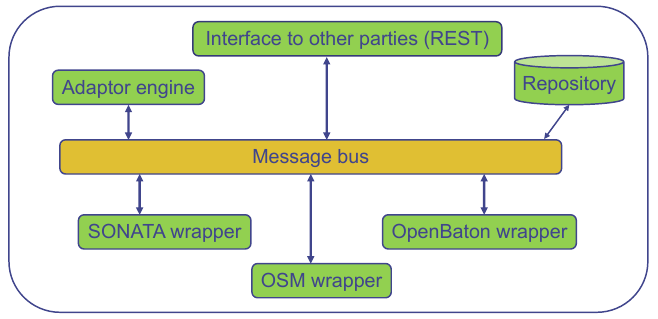
\includegraphics[width=0.9\linewidth]{figures/wp3Arch}
	\caption{Reference architecture for MA \cite{WPDescriptionsPDF}}
	\label{fig:wp3arch}
\end{figure}

\subsection{Prototype implementation of adaptor components}

As a starting point of the prototype, the plan is to choose one of the MANO frameworks listed in the section \ref{manoframeworks} and implement the wrapper for the interfaces provided by it, with focus on modularity and portability. Thereby, making it easy to add support for interfaces provided by other MANO frameworks.

\subsection{Investigation of MANO scalability challenges}
\label{wp3manoresearch}
The plan is to investigate MANO scalability challenges by answering research questions such as the ones listed below but not limited to. (Figure \ref{fig:wp3manoscale})
\begin{itemize}
	\item What is the optimal number of MANO instances in a system?
	\item What is the optimal hierarchical level in a system?
\end{itemize}

\begin{figure}[h]
	\centering
	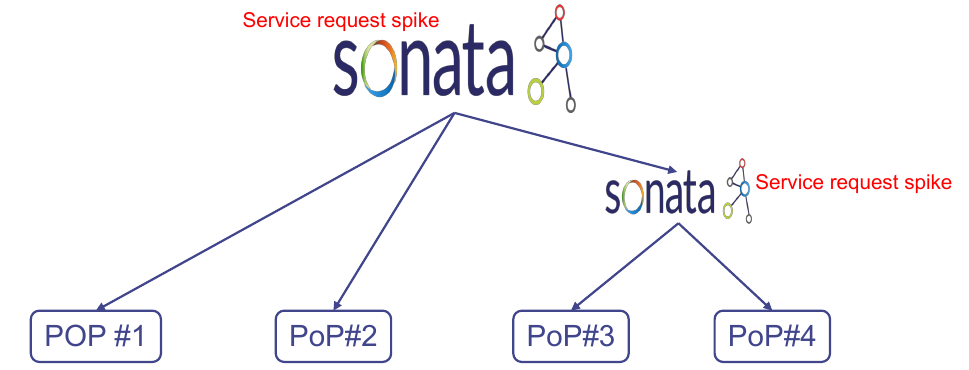
\includegraphics[width=0.9\linewidth]{figures/wp3manoScale}
	\caption{MANO scaling scenario \cite{WPDescriptionsPDF}}
	\label{fig:wp3manoscale}
\end{figure}


\subsection{Proof of concept demonstration}
MA is demonstrated by having two/three virtual machines with MANO frameworks installed, a scenario where a huge number of service requests on one of the MANOs is created. In order to balance the load, the MANO experiencing the service request spike splits the load with another MANO instance. The capability of the MANO to communicate between other MANO instances with the help of MA is thus demonstrated.

\section{Cross-WPs tasks}
\subsection{Requirements definition of WPs integration}
The requirements for this task is to include the functionalities of SDT, SDS and MA to extend the capabilities of a MANO framework.

\subsection{Integration implementation of WPs}
The REST interfaces required for the cross-WP communication are implemented.
The exact idea is unclear at this point in time. 


\subsection{Proof of concept demonstration}
The end-to-end workflow of the software suite is demonstrated. 
